O gerenciamento de requisitos é um processo que consome muitos recursos. neste processo deve-se decidir sobre:

1 - Identificação de requisitos: Cada requisito deve ser identificado unicamente de modo que possa ser feita a referência cruzada entre este e outros requisitos para que ele possa ser utilizado nas avaliações de rastreabilidade.
2 - Processo de gerenciamento de mudanças: É o conjunto de atividades que avaliam o impacto e custo das mudanças.
3 - Políticas de rastreabilidade: Essas políticas definem os relacionamentos entre os requisitos e o projeto do sistema, que devem ser registrados, e como estes registros devem ser mantidos.
3 - Apoio de Ferramentas: O gerenciamento de requisitos envolve o processamento de grandes quantidades de informações sobre os requisitos. As ferramentas que podem ser usadas variam desde sistemas especializados de gerenciamento de requisitos a planilhas  e sistemas simples de banco de dados.
(SOMMERVILLE, 2007, p.108).

\section{Atributos de Requisitos}

Requisitos não são constituídos apenas pela especificação do que é requerido, mas também por um conjunto de informações adicionais que auxiliam a interpretar e gerenciar os requisitos. (25)

Buscando uma melhor forma de gerenciar, foram definidos os atributos que cada requisito deverá conter, e são eles:

1 - Origem

Os requisitos possuirão um código único que será sua identificação.

\begin{table}[]
\centering
\caption{Identificação dos requisitos}
\label{my-label}
\begin{tabular}{|l|l|}
E & Épico \\ \hline
F & Feature \\ \hline
H & User Story \\ \hline
\end{tabular}
\end{table}


2 - Status

Irá indicar o grau de completude do requisito, podendo ser:
Completo: requisito já foi implementado no sistema.

\begin{itemize}
\item Em progresso: requisito está sendo implementado no sistema.
\item Não iniciado: indica que o requisito está no backlog mas não foi implementado ainda.
\end{itemize}

3 - Prioridade

Este atributo indicará o nível de importância para os stakeholders, sistema e outros requisitos.

\begin{itemize}
\item Alta: quando o requisito é de suma importância para os stakeholders ou quando sem ele o sistema não funciona.
\item Média: requisito que é importante para os interessados, mas que ainda sem ele o sistema funciona de forma básica.
\item Baixa: requisito que não compromete o funcionamento do sistema, podendo ser uma funcionalidade opcional.
\end{itemize}

4 - Complexidade

Indica nível de dificuldade para implementar o requisito em questão.

\begin{itemize}
\item Alta: requisito com grau de dificuldade elevado, sendo necessário um grande esforço da equipe para implementação.
\item Média: requisito com grau de dificuldade médio, sendo necessário um esforço da equipe mas de forma moderada.
\item Baixa: requisito com baixo grau de dificuldade de  implementação.
\end{itemize}

5 - Risco

Requisitos que apresentam alguma possibilidade de risco para o sistema durante o desenvolvimento.

\begin{itemize}
\item Alto: requisito com grande possibilidade de risco, necessita de uma atenção maior da equipe.
\item Médio: requisito com média possibilidade de risco.
\item Baixo: requisito com baixa possibilidade de risco.
\end{itemize}

Os requisitos seguirão este padrão:

\begin{table}[\htp]
\centering
\caption{Atributos do Requisito}
\label{my-label}
\begin{tabular}{|l|l|}
\hline
Origem      & E, F ou H                                         \\ \hline
Status    & Completo, em progresso ou não iniciado. \\ \hline
Prioridade & Alta, média ou baixa.\\ \hline
Complexidade & Alta, média ou baixa\\ \hline
Risco  & Alto, médio ou baixo.\\ \hline
\end{tabular}
\end{table}

\section{Rastreabilidade de requisitos}

Segundo Sommerville, “A rastreabilidade é a propriedade de uma especificação de requisitos que reflete a facilidade de encontrar requisitos relacionados”. No conceito de de requisitos de software, diz respeito a capacidade de se acompanhar um requisito em todo seu ciclo de vida, permitindo que se encontre artefatos e outros requisitos que estejam alinhados de alguma forma. É essencial a identificação da composição dos requisitos, das suas dependências entre outros, dos requisitos conflitantes e ainda sua origem e seus interessados, além da identificação de em quais artefatos produzidos o requisito é retratado (27).

Propriedade básica que deve estar presente em todos os tipos de rastreabilidade, de forma a capacitar o completo entendimento das funções, é a capacidade de rastrear para frente (Forwards) e para trás (Backwards), tal que o primeiro permite o rastreio de um requisito até seus refinamentos e  o segundo permite o rastreio dos refinamentos até a sua origem. (28)

Sobre os tipos de rastreabilidade, existem basicamente duas classificações gerais: horizontal e vertical e pré e pós-rastreabilidade. (29)

A rastreabilidade horizontal é entre diferentes versões ou variações de requisitos, ou outros artefatos, em uma fase do ciclo de vida particular. A rastreabilidade vertical é realizada entre requisitos e artefatos produzidos pelo processo de desenvolvimento ao longo do ciclo de vida do projeto.
Uma visão simplificada sobre os tipos de rastreabilidade é apresentada na Figura a seguir (30):

\FloatBarrier
\begin{figure}[!htpd]
		\centering
		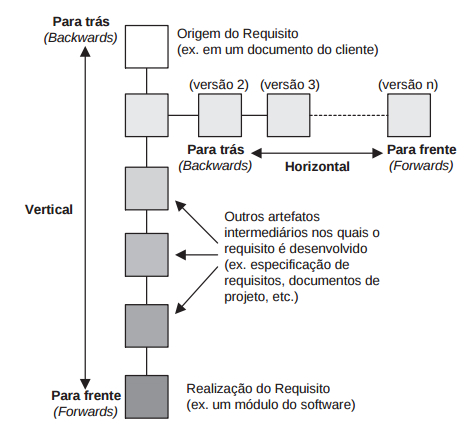
\includegraphics[scale=0.8]{figuras/Rastreabilidade}
		\label{img:SAF}
		\caption{Rastreabilidade}
\end{figure}
\FloatBarrier

A segunda classe de rastreabilidade trata da pré-rastreabilidade, que está concentrada no ciclo de vida dos requisitos antes de serem incluídos no processo de especificação, e a pós-rastreabilidade, que está concentrada no ciclo de vida dos requisitos após serem incluídos na especificação de requisitos. A imagem a seguir ilustra a pré e pós-rastreabilidade (30):


\FloatBarrier
\begin{figure}[!htpd]
		\centering
		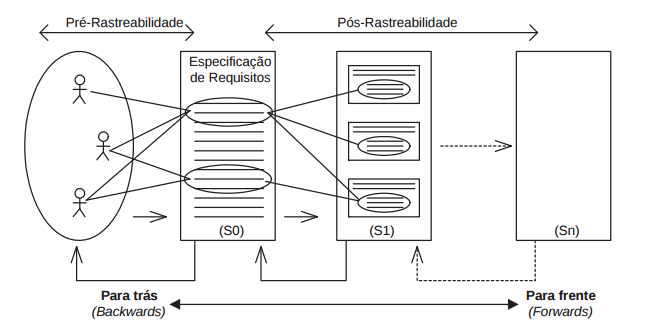
\includegraphics[scale=0.8]{figuras/rastrabilidadepre}
		\label{img:SAF}
		\caption{Pré-rastreabilidade}
\end{figure}
\FloatBarrier

Tomando por base os conceitos citados, foi adotado pelo grupo um modelo de rastreabilidade bi-direcional, que visa garantir o completo rastreio desde os Temas de Investimento até as Tarefas de cada História. Tais requisitos serão identificados da seguinte forma:

\begin{table}[\htp]
\centering
\caption{Rastreabilidade}
\label{my-label}
\begin{tabular}{|l|l|l|}
Sigla & Descrição & Exemplo \\ \hline
T & Tema de Investimento & T01 \\ \hline
T & Tema de Investimento & T01 \\ \hline
E & Épico & T02E03 \\ \hline
F & Feature & T01E02F05 \\ \hline
H & História & T01E02F05H12 \\ \hline
TR & Tarefa & T01E02F05H12TR09 \\ \hline
\end{tabular}
\end{table}

A representação em mapa destes requisitos é dada da seguinte forma:

\FloatBarrier
\begin{figure}[!htpd]
		\centering
		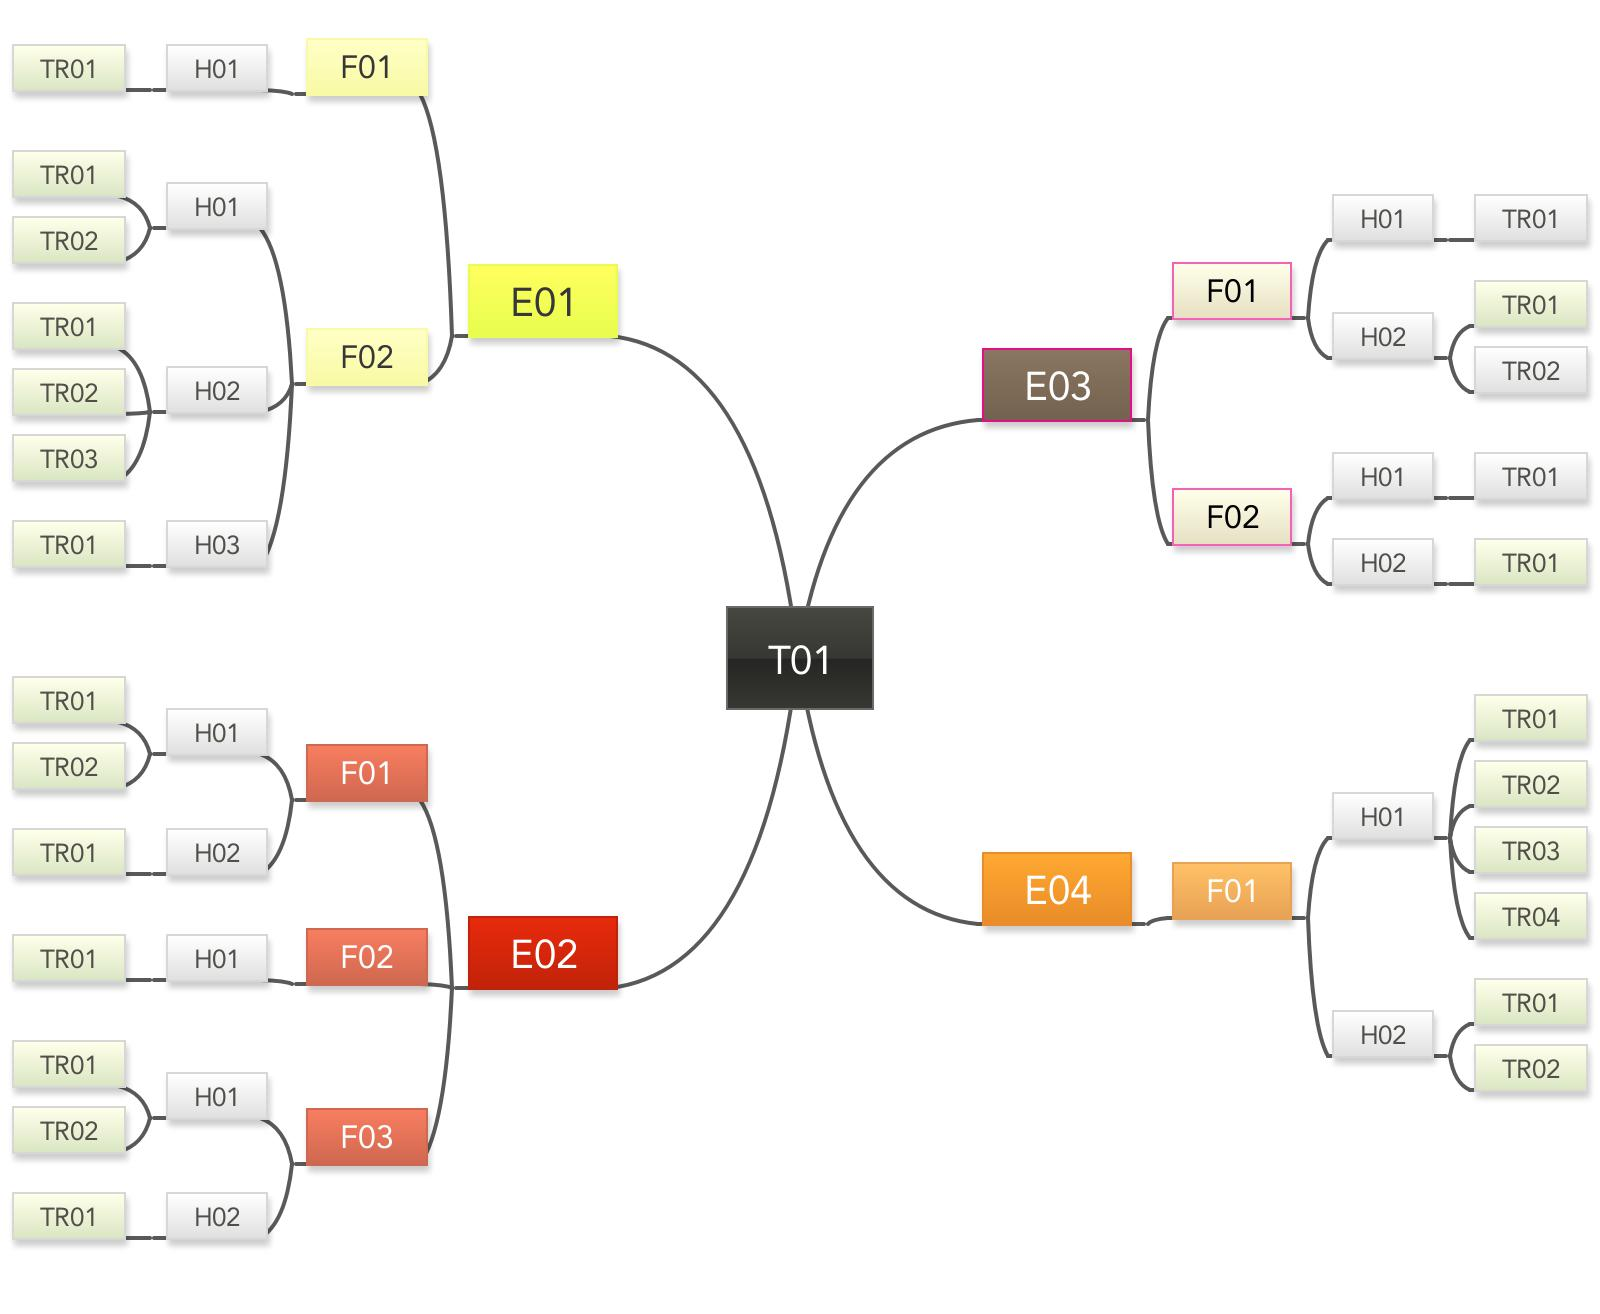
\includegraphics[scale=0.27]{figuras/T01}
		\label{img:SAF}
		\caption{Mapa Requisitos}
\end{figure}
\FloatBarrier
